\documentclass{beamer}

\usepackage[utf8]{inputenc}
\usepackage[frenchb]{babel}
\usepackage{verbatim}
\usepackage{graphicx}
\usepackage{color}
\usepackage{hyperref}
\usepackage{verbatim}
\usepackage{url}
\usepackage{moreverb}
\usepackage{fancyvrb}
\usepackage{minted}
\usepackage{algpseudocode}
\usepackage{natbib}
\usepackage{eulervm}
\usepackage{auto-pst-pdf}
\usepackage{pst-plot}
\usepackage{multirow}
\usepackage{subfigure}


\hypersetup{colorlinks=true, linkcolor=black, urlcolor=blue}
\usetheme{boxes}
\beamertemplatenavigationsymbolsempty
\setbeamertemplate{sections/subsections in toc}[circle]
\setbeamertemplate{footline}[frame number]
\setbeamertemplate{itemize items}[circle]
\setbeamertemplate{itemize subitem}[square]

\title{{\bf A workflow for large-scale computer-aided cytology and its applications}}
\author{Romain Mormont}
\institute{Université de Liège, Belgium}
\date{June 22, 2016}

\newcommand{\todo}[1]{\textcolor{red}{[TODO] #1}}

\definecolor{lightgreen}{rgb}{0.0,0.8,0.0}
\definecolor{lightblue}{rgb}{0.3,0.8,1.0}
\definecolor{lightred}{rgb}{0.874,0.180,0.105}
\definecolor{gray}{rgb}{0.4,0.4,0.4}
\definecolor{lightgray}{rgb}{0.8,0.8,0.8}
\definecolor{shadecolor}{rgb}{0.9,0.9,0.9}
\newrgbcolor{mygreen}{.00 .5 .00}
\newrgbcolor{myyellow}{.6 .6 .00}

\DeclareMathOperator*{\argmax}{arg\,max}


\newrgbcolor{mygreen}{.00 .5 .00}
\newcommand{\X}[1]{\textcolor{blue}{#1}}
\newcommand{\y}[1]{\textcolor{red}{#1}}
\newcommand{\model}[1]{\textcolor{mygreen}{#1}}
\newcommand{\loss}[1]{\textcolor{lightblue}{#1}}

\begin{document}
\setbeamertemplate{caption}{\raggedright\insertcaption\par}
\renewcommand{\inserttotalframenumber}{17}

% Title page ==================================================================

\begin{frame}
\titlepage
\begin{center}
	\footnotesize
	\textit{Supervisor}: Dr. Raphaël Marée\\
	\textit{Academic}: Pr. Pierre Geurts
\end{center}
\end{frame}


\begin{frame}{Context and application}
	\vfill
	\begin{figure}[h]
	\center
	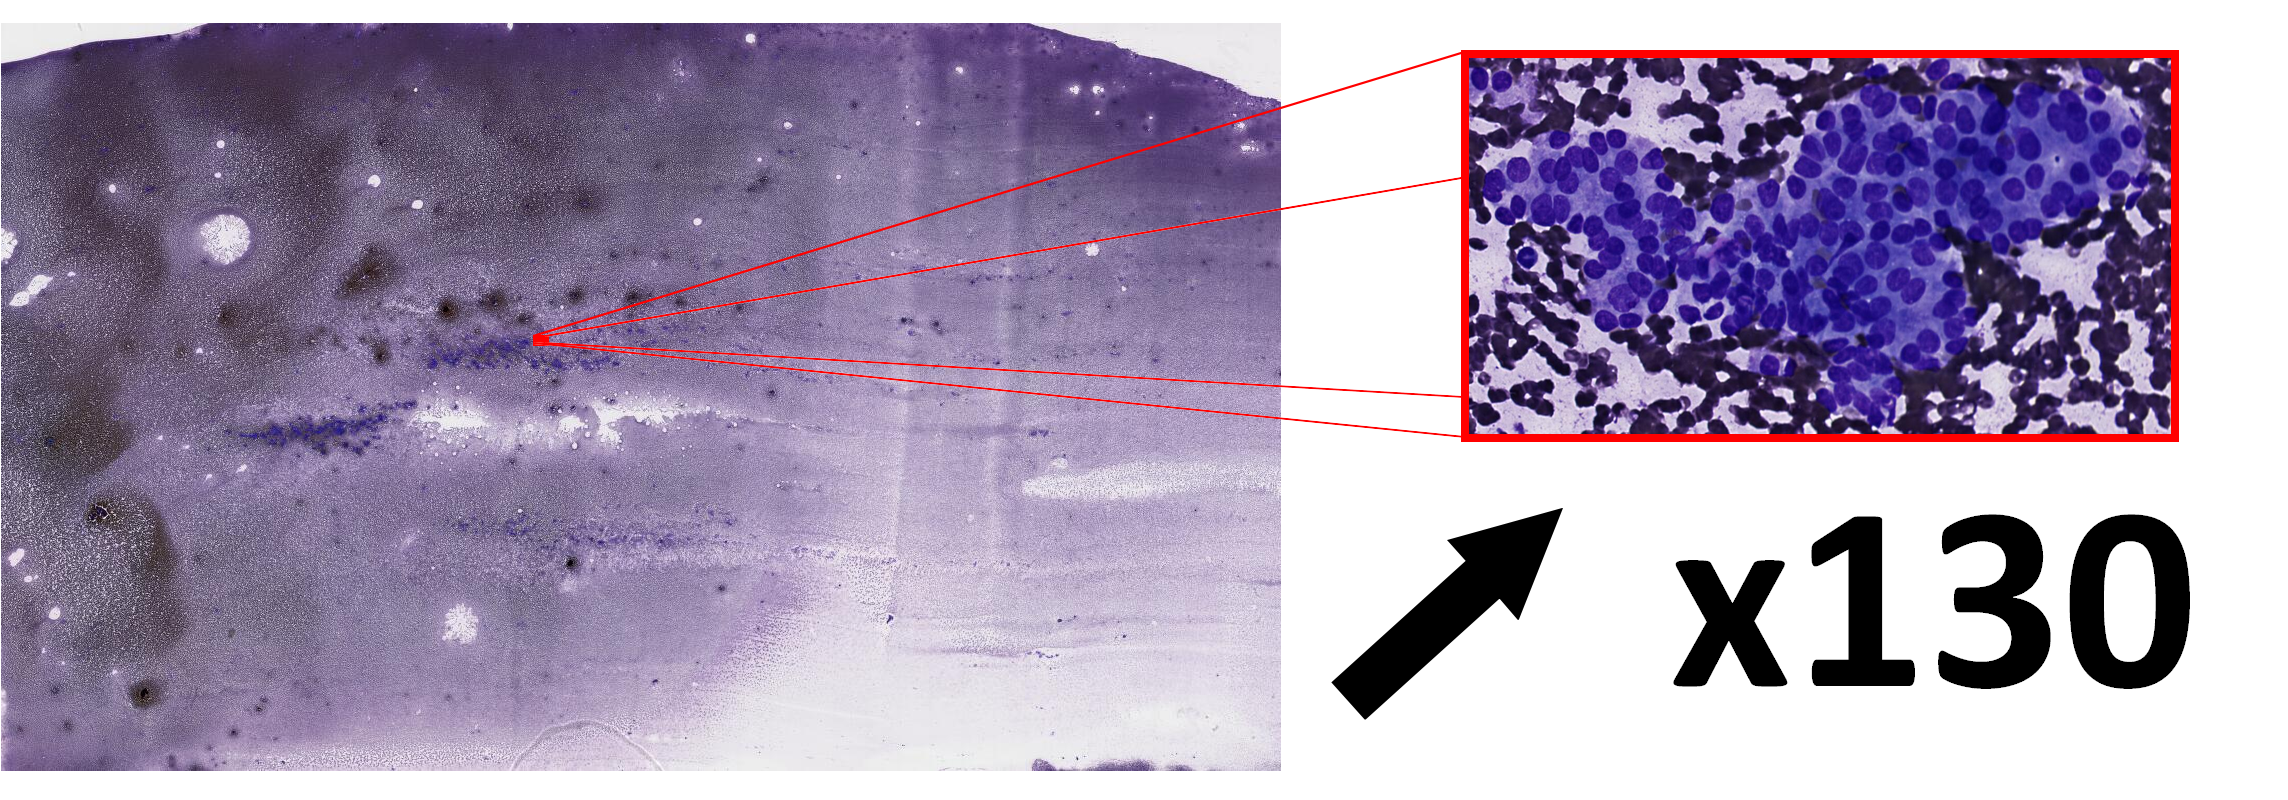
\includegraphics[scale=0.17]{images/whole-slide-dim.png}
	\caption{Microscope slide smeared with cell samples (15 gigapixels).}
	\end{figure}
	\vfill
\end{frame}


\begin{frame}{Application: thyroid nodule malignancy}
	\begin{figure}
		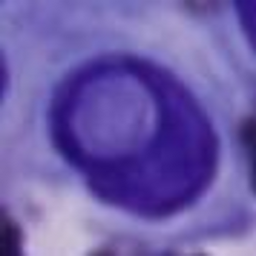
\includegraphics[scale=0.3]{images/incl1.png}
		\hspace{1cm}
		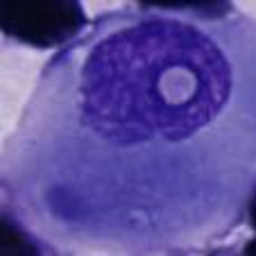
\includegraphics[scale=0.3]{images/incl2.png}
	\end{figure}
	\begin{figure}
		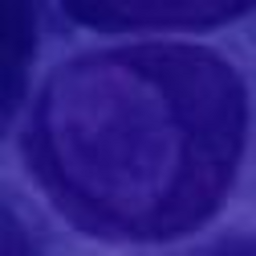
\includegraphics[scale=0.3]{images/incl3.png}
		\hspace{1cm}		
		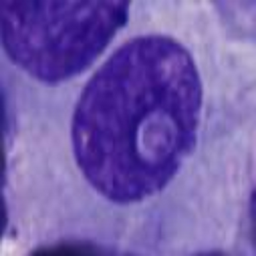
\includegraphics[scale=0.3]{images/incl4.png}
		\caption{Cells with inclusion}
	\end{figure}
\end{frame}


\begin{frame}{Application: thyroid nodule malignancy}
	\begin{figure}
		\center
		\subfigure[Proliferative]{
			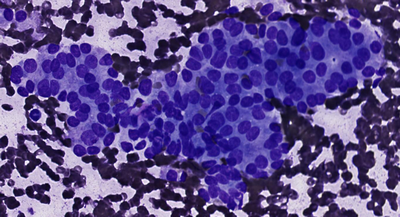
\includegraphics[scale=0.35]{images/prolif_pattern_1.png}
			\hspace{1cm}
			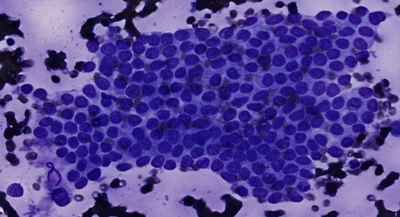
\includegraphics[scale=0.35]{images/prolif_pattern_2.png}
			\label{sfig:prolif_patterns}
		} \\
		\subfigure[Non-proliferative]{
			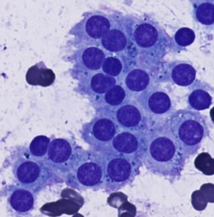
\includegraphics[scale=0.35]{images/normal_pattern_1.png}
			\hspace{1cm}
			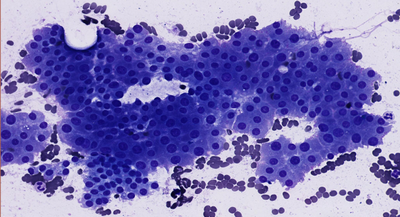
\includegraphics[scale=0.35]{images/normal_pattern_2.png}
			\label{sfig:norm_patterns}
		}
		\caption{Architectural patterns}
	\end{figure}
\end{frame}


\begin{frame}{Application: thyroid nodule malignancy}
	\begin{center}
		\Large
		Can be expressed as a problem of \textbf{object detection and classification} !
	\end{center}	
\end{frame}

\begin{frame}{Objectives}

	\begin{enumerate}
		\item \textbf{Developing a framework} for performing object detection and classification in multi-gigapixel images
		\vspace{1cm}
		\item \textbf{Applying this framework} to the problem of thyroid malignancy diagnosis
	\end{enumerate}

\end{frame}


\begin{frame}{SLDC framework}
	\textbf{Technical challenges}:
	\begin{itemize}
		\item Memory constraint (images do not fit into memory)
		\item Efficiency
		\item Parallelism
		\item Genericity
	\end{itemize}
\end{frame}


\begin{frame}{SLDC framework: algorithms (workflow)}
	\begin{figure}
		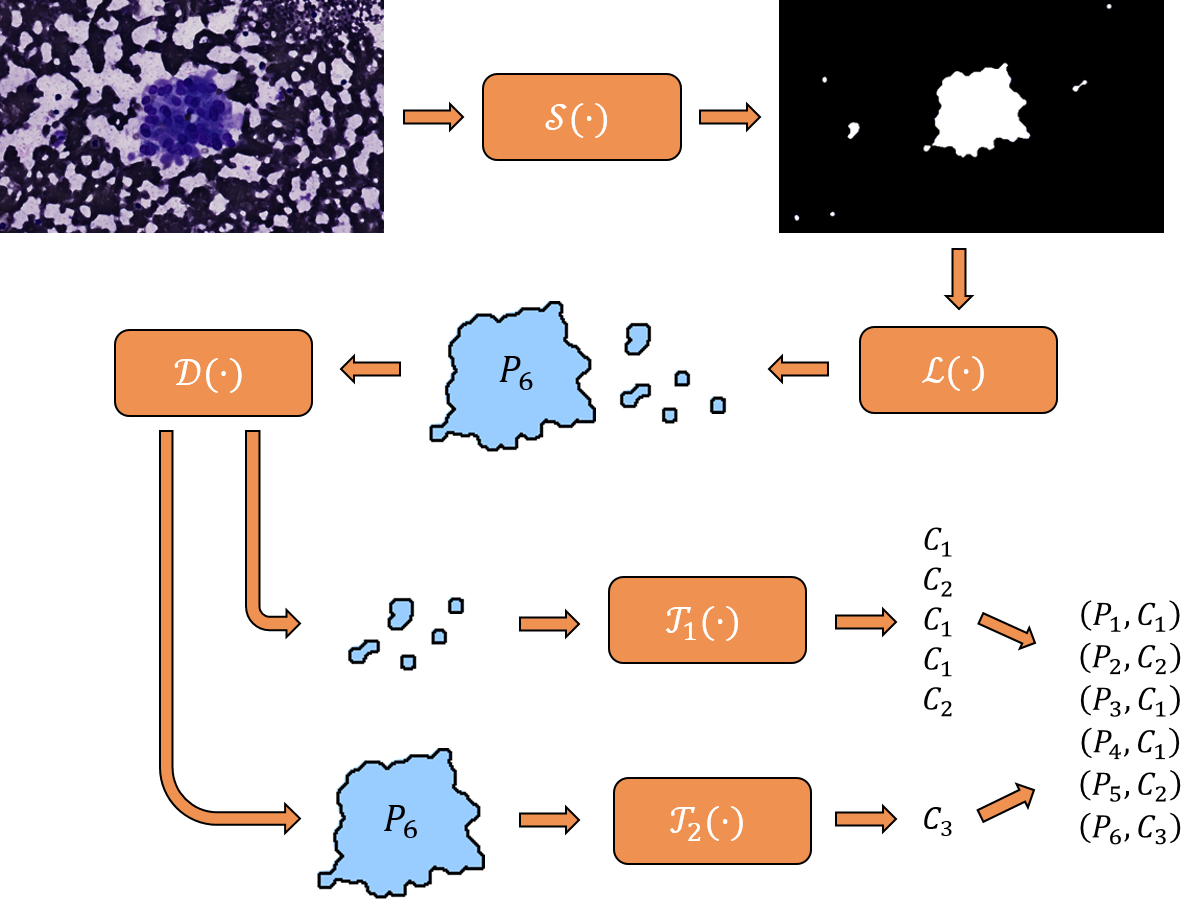
\includegraphics[scale=0.45]{images/workflow_illustration.png}
	\end{figure}
\end{frame}


\begin{frame}{SLDC framework: implementation}
	Key features:
	\begin{itemize}
		\item Memory constraint handled by \textbf{splitting images into tiles}
		\item Customizable \textbf{logging system} allowing user to keep track of execution progress
		\item \textbf{Several levels of parallelism} available 
		\item \textbf{Builder components} providing an easy way of building complex workflows
	\end{itemize}
	\vspace{0.5cm}
	About the implementation: 
	\begin{itemize}
		\item Implemented as a Python library
		\item Available on GitHub at {\small\url{https://github.com/waliens/sldc}}
		\item Unit-tested (coverage of 85 \%)
		\vspace{0.5cm}
	\end{itemize}
\end{frame}


\begin{frame}{SLDC at work}
	\begin{center}	
		Aim: detect \textbf{cells with inclusion} and \textbf{proliferative architectural patterns}
	\end{center}
	\begin{figure}
		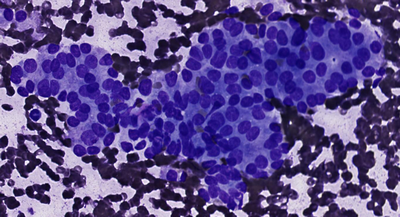
\includegraphics[scale=0.55]{images/prolif_pattern_1.png}
		\hspace{1cm}
		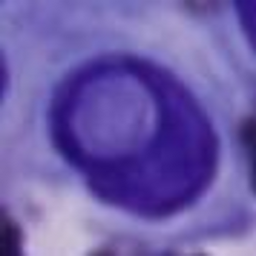
\includegraphics[scale=0.35]{images/incl1.png}
	\end{figure}
\end{frame}


\begin{frame}{SLDC at work: slide processing}
	\begin{figure}
		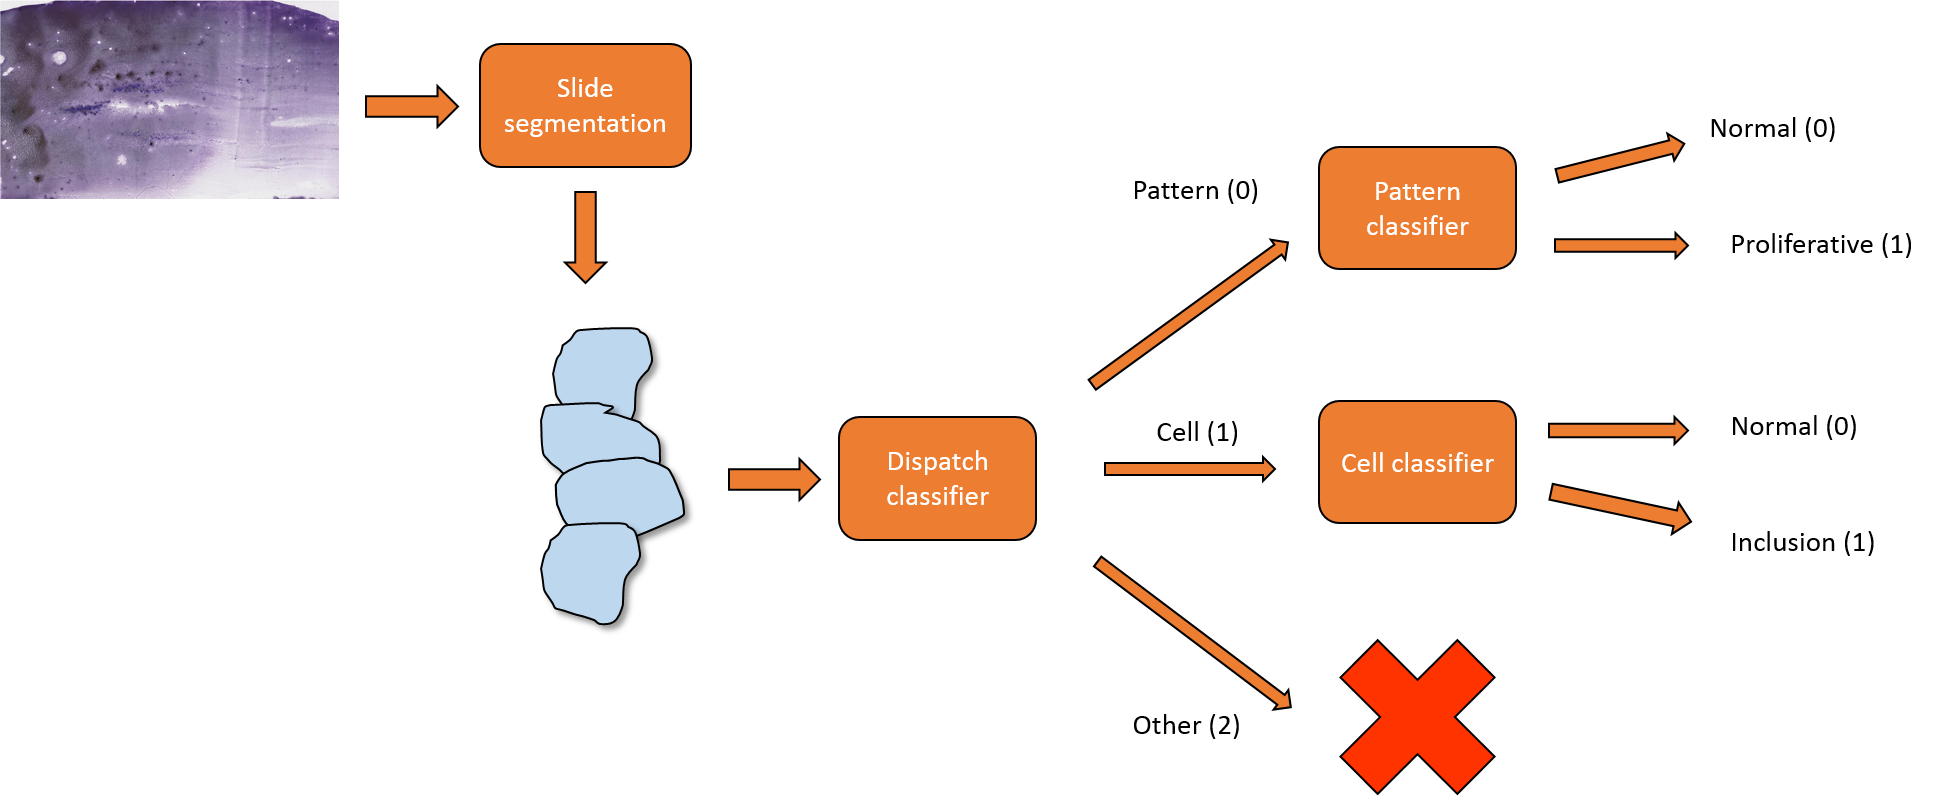
\includegraphics[scale=0.35]{images/thyroid_workflow_1.png}
	\end{figure}
\end{frame}


\begin{frame}{SLDC at work: pattern processing}
	\begin{figure}
		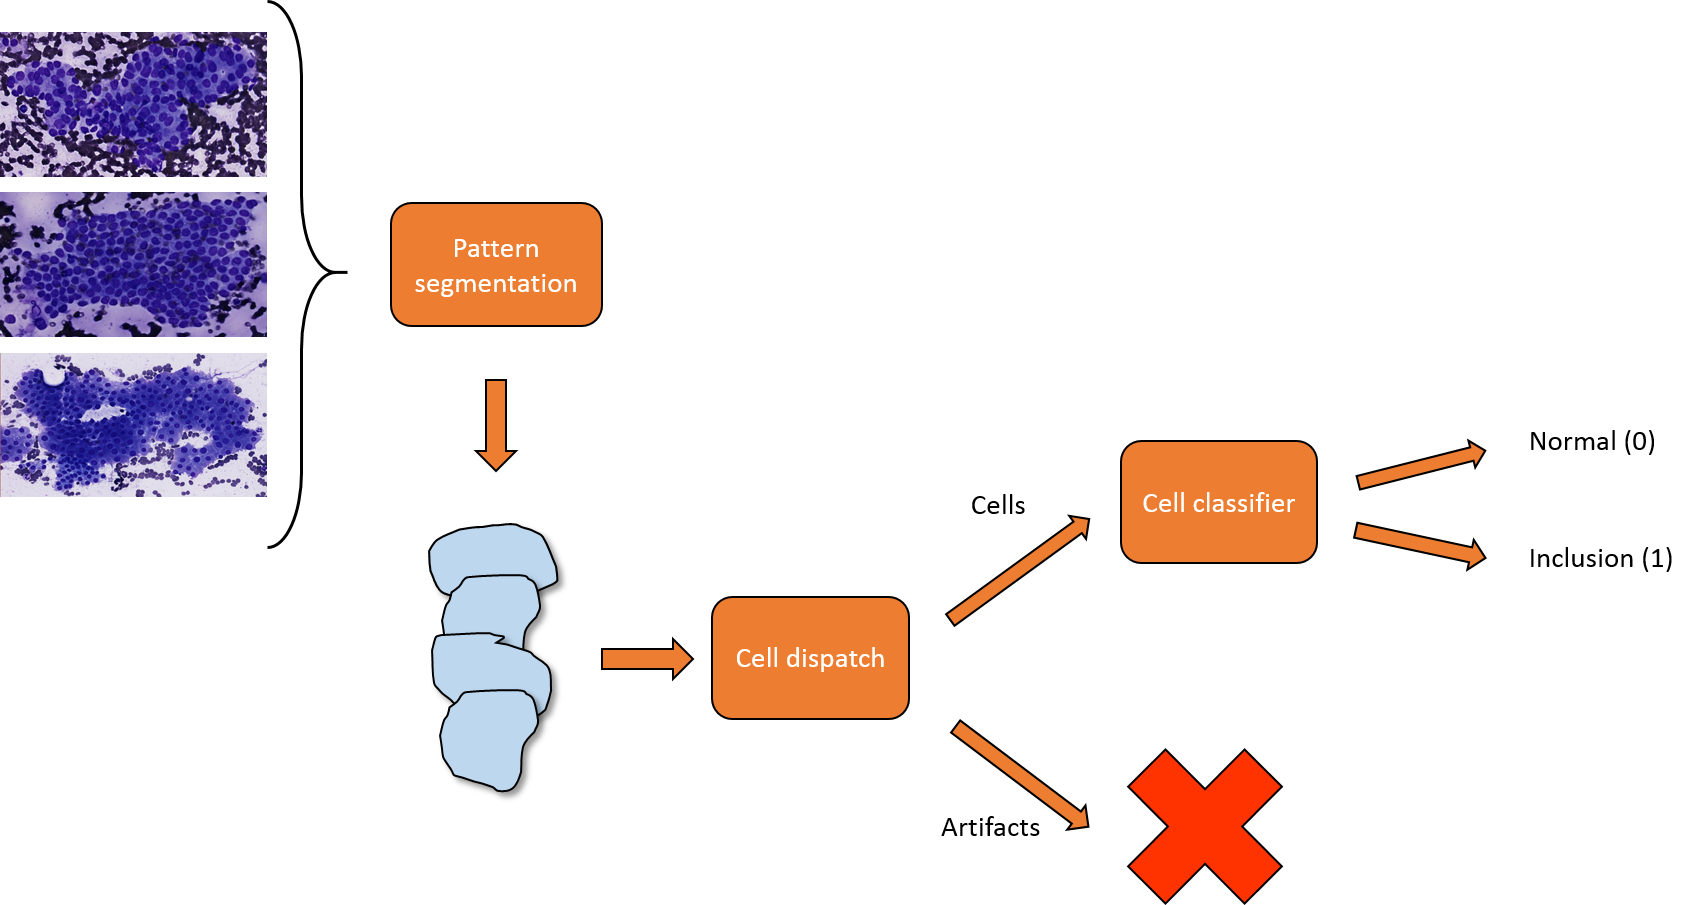
\includegraphics[scale=0.4]{images/thyroid_workflow_2.png}
	\end{figure}
\end{frame}


\begin{frame}{SLDC at work: execution times}
	\begin{itemize}
		\item Execution times mostly dominated by network communication
		\item Effective time for 16 giga-pixels images is 18 minutes
		\item \textbf{Effective time for 8 giga-pixels images is 8 minutes}
	\end{itemize}
	
	\begin{figure}
		\subfigure[Acceleration brought by using more processes.]{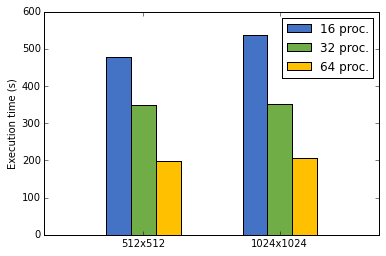
\includegraphics[scale=0.35]{images/perf_lsl_parallelization.png}}
		\hspace{0.5cm}
		\subfigure[Scalability of the LSL phase.]{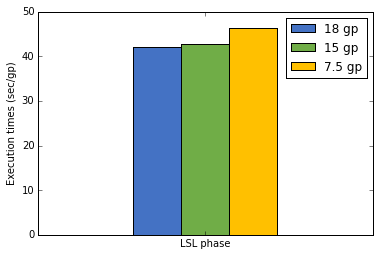
\includegraphics[scale=0.35]{images/perf_lsl_sec_gp.png}}
	\end{figure}
\end{frame}


\begin{frame}{SLDC at work: detection}
	\begin{figure}
		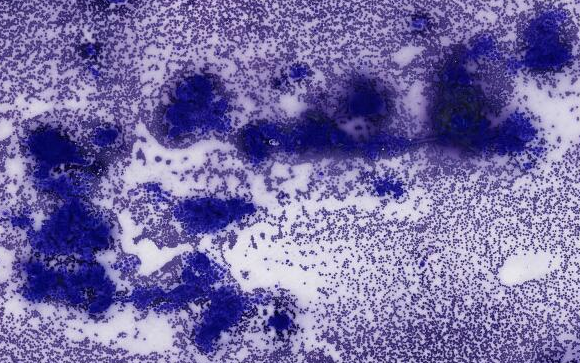
\includegraphics[scale=0.3]{images/success_pattern_1_nopat.png}
		\hspace{0.25cm}
		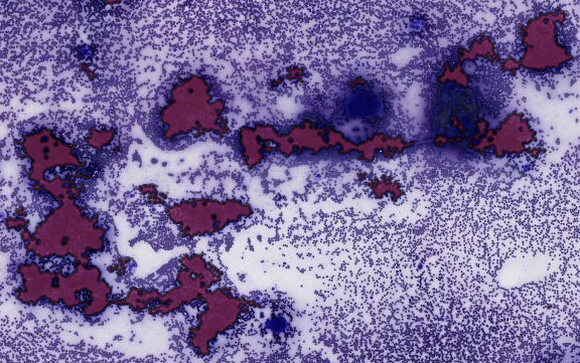
\includegraphics[scale=0.3]{images/success_pattern_1_pat.png}\\
		\vspace{0.25cm}
		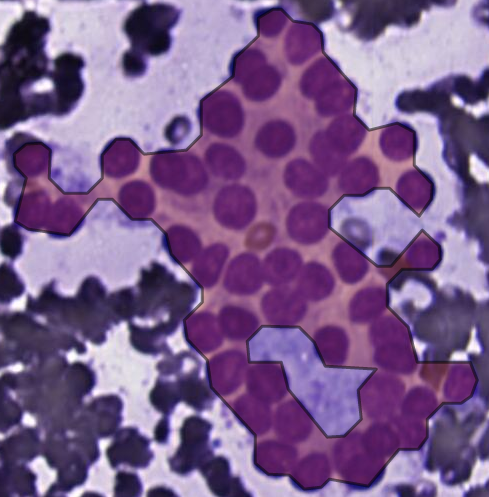
\includegraphics[scale=0.25]{images/success_reseg_2_pat.png}
		\hspace{1cm}
		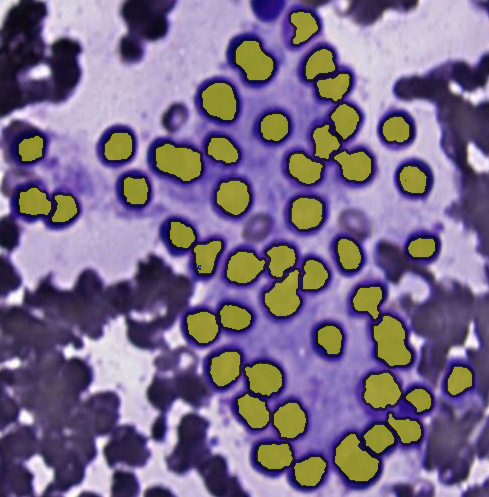
\includegraphics[scale=0.25]{images/success_reseg_2_nopat.png}
	\end{figure}
\end{frame}

\begin{frame}{Conclusions}
	\begin{enumerate}
		\item The \textbf{framework is production-ready} and available on GitHub.
		\vspace{1cm}
		\item The implemented workflow provides \textbf{promising results} but \textbf{still requires some improvements}.
	\end{enumerate}
\end{frame}

\begin{frame}{Future works}

	\begin{block}{SLDC framework}
		\begin{itemize}
			\item Was \textbf{improved since the master thesis submission} (parallelization, ease of use,...).
			\item But some minor improvements must still be performed.
		\end{itemize}
	\end{block}
	
		
	\begin{block}{Thyroid workflow}
		\begin{itemize}
			\item Improving the segmentation procedures
			\item Improving the classification models
		\end{itemize}
	\end{block}
\end{frame}

\begin{frame}
	\vfill
	\begin{center}
		Thank you for your attention ! \\
		Any question ?
	\end{center}
	\vfill
\end{frame}

\end{document}